\documentclass{article}

\usepackage[utf8]{inputenc}
\usepackage[french]{babel}
\usepackage[top=3cm, bottom=3cm, left=3cm, right=3cm]{geometry}
\usepackage{graphicx}
\usepackage{array}
\usepackage[T1]{fontenc}
\usepackage{tikz}
\usepackage{hyperref}
\usepackage[underline=true,rounded corners=false]{pgf-umlsd}
\usepackage{listings}
\usepackage{color}

\title{\textbf{Rapport projet spécif}}
\author{Ilyas TOUMLILT\\Massine BITAM}
\begin{document}
\maketitle
\section{Cas 1: Système mono processeur}
\begin{sequencediagram}
  
	\newinst[2]{p}{processeur}
	\newinst[2]{c}{cache}
	\newinst[2]{a}{arbitre / bus}
	\newinst[2]{m}{mémoire}
	
\begin{sdblock}{Pa1}{}
	\mess[1]{p}{CPU Read [0]}{c}
	\prelevel
	\mess[1]{c}{gel}{p}
	\prelevel\prelevel
	\mess[1]{c}{}{a}
	\prelevel
	\mess[1]{a}{Read[0]}{m}
	\prelevel
	\mess[1]{m}{Data[0]}{a}
	\prelevel
	\mess[1]{a}{Data[0]}{c}
	\prelevel
	\mess[1]{c}{Data[0]}{p}
	
	\begin{callself}{p}{add, R1, R1,1}{}
	\end{callself}
	\mess[1]{p}{CPU WR [1]}{c}
	\prelevel
	\mess[1]{c}{gel}{p}
	\prelevel\prelevel
	\mess[1]{c}{}{a}\prelevel\mess[1]{a}{Write[1]}{m}
	\mess[1]{m}{}{a}\prelevel\mess[1]{a}{}{c}\prelevel\mess[1]{c}{écriture términé}{p}
	
	\mess[1]{p}{CPU Read [0]}{c}
	\prelevel
	\mess[1]{c}{Data[0]}{p}
	\begin{callself}{p}{add, R2, R2}{}
	\end{callself}
	
	\mess[1]{p}{CPU WR [0]}{c}
	\prelevel
	\mess[1]{c}{gel}{p}
	\prelevel\prelevel
	\mess[1]{c}{}{a}\prelevel\mess[1]{a}{Write[0]}{m}
	\mess[1]{m}{}{a}\prelevel\mess[1]{a}{}{c}\prelevel\mess[1]{c}{écriture términé}{p}
\end{sdblock}
\end{sequencediagram}
\\Après eviction du cache voici le diagramme de séquence du programme P1b.\\
\begin{sequencediagram}
	\newinst[2]{p}{processeur}
	\newinst[2]{c}{cache}
	\newinst[2]{a}{bus}
	\newinst[2]{m}{mémoire}
	
\begin{sdblock}{P1b}{}
	\mess[1]{p}{CPU Read [0]}{c}
	\prelevel
	\mess[1]{c}{gel}{p}
	\prelevel\prelevel
	\mess[1]{c}{}{a}
	\prelevel
	\mess[1]{a}{Read[0]}{m}
	\prelevel
	\mess[1]{m}{Data[0]}{a}
	\prelevel
	\mess[1]{a}{Data[0]}{c}
	\prelevel
	\mess[1]{c}{Data[0]}{p}
	
	\mess[1]{p}{CPU Read [1]}{c}
	\prelevel
	\mess[1]{c}{gel}{p}
	\prelevel\prelevel
	\mess[1]{c}{}{a}
	\prelevel
	\mess[1]{a}{Read[1]}{m}
	\prelevel
	\mess[1]{m}{Data[1]}{a}
	\prelevel
	\mess[1]{a}{Data[1]}{c}
	\prelevel
	\mess[1]{c}{Data[1]}{p}
	
	\begin{callself}{p}{add, R3, R1,R2}{}
	\end{callself}
	\mess[1]{p}{CPU WR [0]}{c}
	\prelevel
	\mess[1]{c}{gel}{p}
	\prelevel\prelevel
	\mess[1]{c}{}{a}\prelevel\mess[1]{a}{Write[1]}{m}
	\mess[1]{m}{}{a}\prelevel\mess[1]{a}{}{c}\prelevel\mess[1]{c}{écriture términé}{p}
	
\end{sdblock}
\end{sequencediagram}
\newpage
Voici l'architecture de notre Système mono-processeur ansi que les connections des differant composant.\\
\begin{center}
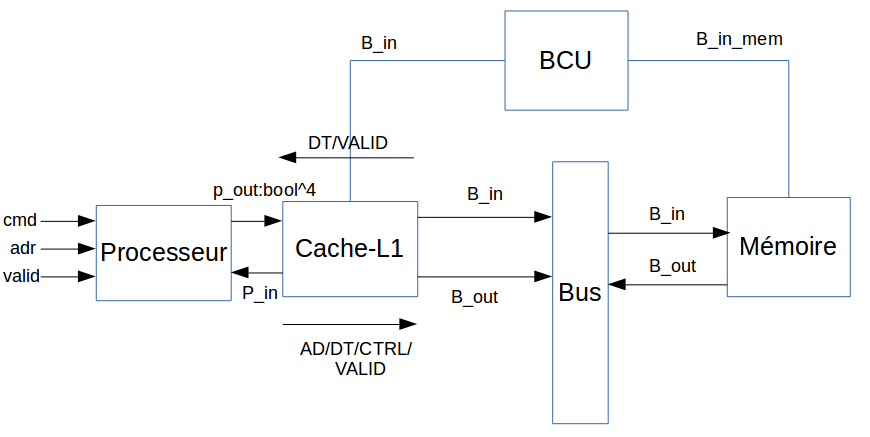
\includegraphics[scale=0.5]{mono.png} 
\end{center}


\newpage
\section{Cas 2: Système multi processeur}
\begin{sequencediagram}
  
	\newinst[0]{p1}{proc1}
	\newinst[0]{c1}{cache1}
	\newinst[1]{p2}{proc2}
	\newinst[0]{c2}{cache2}
	\newinst[1]{a}{arbitre}
	\newinst[1]{b}{bus}
	\newinst[1]{m}{mémoire}
\begin{sdblock}{partage en lecture}{une écriture}	
	\mess{p1}{CPU Read [0]}{c1}\prelevel
	 \mess{p2}{CPU Read [0]}{c2}\prelevel
	 \mess[1]{c1}{}{a}
	 \prelevel\prelevel
	\mess[1]{c2}{}{a}\prelevel
	\mess[1]{a}{READ P1[0]}{b}\prelevel
	\mess[1]{b}{READ P1[0]}{m}\prelevel
	 \mess[1]{m}{DATA P1 [0]}{b}\prelevel
	 \mess[1]{b}{DATA P1 [0]}{c1}\prelevel
	 \mess{c1}{DATA P1 [0]}{p1}
	 \begin{callself}{p1}{add, R3, R1,1}{}
	 \end{callself}\prelevel
	 \mess[1]{a}{READ P2[0]}{b}\prelevel
	 \mess[1]{b}{READ P2[0]}{m}\prelevel
	 \mess[1]{m}{DATA P2[0]}{c2}\prelevel
	 \mess{c2}{DATA P2 [0]}{p2}\prelevel
	 \mess{p1}{CPU WRITE [0]}{c1}\prelevel
	 \mess[1]{c1}{}{a}\prelevel
	  \begin{callself}{p2}{...}{}
	 \end{callself}\prelevel\prelevel
	 \mess[1]{a}{Store P1 [0]}{b}\prelevel
	 \mess[1]{b}{Store P1 [0]}{m}\prelevel
	 \mess[1]{m}{Store Done}{b}\prelevel
	 \mess[1]{b}{Store Done}{c1}\prelevel\prelevel
	 \mess[0]{b}{update value}{c2}
	  \begin{callself}{p1}{...}{}
	 \end{callself}\prelevel\prelevel
	 \begin{callself}{p2}{...}{}
	 \end{callself}
	 \begin{callself}{p2}{ADD R2,  R1, 1}{}
	 \end{callself}
	  \mess{p2}{CPU WRITE [0]}{c2}\prelevel
	 \mess[1]{c2}{}{a}\prelevel
	 \mess[1]{a}{Store P2 [0]}{b}\prelevel
	 \mess[1]{b}{Store P2 [0]}{m}\prelevel
	 \mess[1]{m}{Store Done}{b}\prelevel
	 \mess[1]{b}{Store Done}{c2}
	 \end{sdblock}
\end{sequencediagram}

\newpage
Voici l'architecture de notre Système Multi-processeur ainsi que les connections des différant composant.\\
\begin{center}
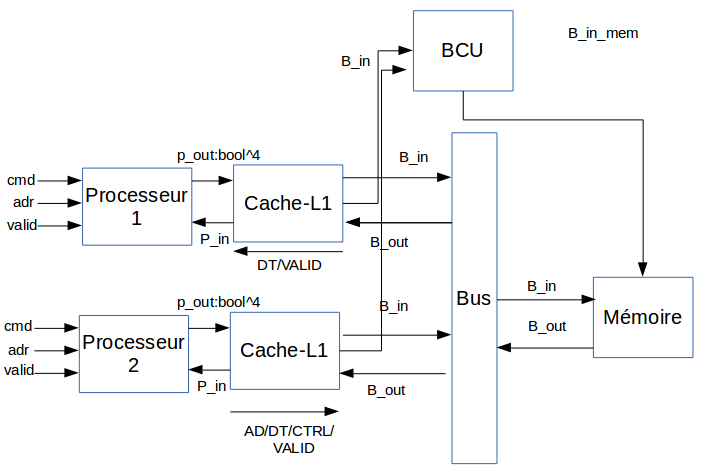
\includegraphics[scale=0.5]{multi.png} 
\end{center}

\newpage
\section{Realisation de la platforme: description des composants}
\textbf{Les requetes :}\\
De type bool\^4 dont les composants sont les suivants :\\
0: AD, adresse du mot à transmettre.\\
1: DT, valeur du mot transmis.\\
2: CTRL, sens de transfert.\\
3: VALID, si les données sont significatives.\\
NB: à partir de là, nous considérons que le terme requête fait référence à ce type de strucuture de données.
\\
\textbf{Le processeur :}\\
Le processeur reçoit en entrée des requêtes du cache ou du cmd ( main ), le signal src gère la source de la requête. Il émet donc selon la source et le type des données une réponse vers un récepteur ( cmd / cache ) géré par le signal de sortir trg. Le proc peut être gelé en cas de MISS sur le cache ( signal de sortie gel ).\\
Comportements du proc :\\
--> à la réception d'une requête cmd : si c'est une requête significative ( VALID ), et que le proc n'est pas gelé, cette requête sera transmise au cache, qui pourra ou non geler le proc selon la disponibilité de la donnée en cache. sinon si ce n'est pas une requête significative, on redirige simplement l'entrée en sortie. si le proc est gelé il ne traite pas la commande.
--> à la réception d'une requête du cache : cette requête peut ou être une requête de gel, qui ne fait que geler le proc en attendant la réponse. Ou une réponse à la requête, qui sera donc redirigée en sortie.\\
\\
\textbf{Le cache :}\\
Le cache stocke le mot préalablement demandé en lecture par le processeur auquel il est associé, jusqu'à ce que ce mot soit mis à jour ou évincé. On a supposé que le cache ne peut contenir qu'un seul mot à la fois.\\
Le cache reçoit plusieurs signaux en entrée :\\
- arb\_gnt : la décision de l'arbitre, et si oui ou non on a droit sur le bus.\\
- l1\_in : requête du proc\\
- b\_out : sortie du bus\\
Il retourne les signaux suivants en sortie :\\
- req : si le cache est demandeur de bus.\\
- gel : s'il le cache veut geler le proc.\\
- l1\_out : request vers proc\\
- b\_in : request vers bus\\
\\
\textbf{Le bus :}\\
Le bus interconnecte la mémoire et les caches L1 des processeurs.\\
son architecture est multipléxée.\\
Le noeud reçoit la décision de l'arbitre et les sorties des caches et de la mémoire\\
Il retourne l'entrée du composant abr\_gnt.\\
\\
\textbf{L'arbitre :}\\
L'arbitre définit, lorsqu'il y a plusieurs requêtes simultannées vers la mémoire, celle qui a la priorité d'accès sur le bus.\\
\\
\textbf{La mémoire :}\\
Composée de NWORDS mots de NBITS bits, adressable par mot.\\
La memoire est interfacée dans le bus et agit sur sollicitation de requêtes d'un des deux caches : \\
----> READ(ad) : demande de lecture du mot d'adresse ad.\\
--    params   : gnt\_mem      = true\\
--               b\_out[CTRL]  = false\\
--               b\_out[AD]    = ad du mot\\
--               b\_out[VALID] = true\\
--    returns  : b\_in[AD]    = b\_out[AD]\\
--               b\_in[DT]    = données demandée\\
--               b\_in[CTRL]  = b\_out[CTRL]\\
--               b\_in[VALID] = true\\
----> WRITE(ad, val) : demande d'écriture de la valeur val à l'adresse ad\\
--    params   : gnt\_mem      = true\\
--               b\_out[AD]    = ad du mot\\
--               b\_out[DT]    = valeur à écrire\\ 
--               b\_out[CTRL]  = true\\
--               b\_out[VALID] = true\\
--    returns  : b\_in[AD]    = b\_out[AD]\\
--               b\_in[DT]    = b\_out[DT]\\
--               b\_in[CTRL]  = b\_out[CTRL]\\
--               b\_in[VALID] = b\_out[VALID]\\
----> Dans tous les autres cas ( cycles d'inactivité on va dire )\\
--    returns  : b\_in[AD]    = b\_out[AD]\\
--               b\_in[DT]    = b\_out[DT]\\
--               b\_in[CTRL]  = b\_out[CTRL]\\
--               b\_in[VALID] = false

\end{document}
